\documentclass[aspectratio=169,10pt]{beamer}
\usetheme{Madrid}
\usecolortheme{default}

\usepackage{hyperref}
\usepackage{tikz}
\usetikzlibrary{patterns,shapes,arrows,calc,positioning,decorations.markings}
\usepackage{circuitikz}
\usepackage{amsmath,amssymb}
\usepackage{graphicx}
\usepackage{listings}
\usepackage{booktabs}

% --- Custom Colors UNIB ---
\definecolor{unibblue}{RGB}{0, 32, 96}
\definecolor{unibgold}{RGB}{197, 160, 89}
\definecolor{unibgreen}{RGB}{34, 112, 60}

\setbeamercolor{palette primary}{bg=unibblue,fg=white}
\setbeamercolor{palette secondary}{bg=unibblue!85,fg=white}
\setbeamercolor{palette tertiary}{bg=unibblue!70,fg=white}
\setbeamercolor{structure}{fg=unibblue}
\setbeamercolor{titlelike}{parent=structure,bg=unibblue,fg=white}
\setbeamercolor{block title}{bg=unibblue!90,fg=white}
\setbeamercolor{block body}{bg=unibblue!8,fg=black}
\setbeamercolor{alertblock title}{bg=unibgold!95,fg=black}
\setbeamercolor{alertblock body}{bg=unibgold!15,fg=black}
\setbeamercolor{exampleblock title}{bg=unibgreen!90,fg=white}
\setbeamercolor{exampleblock body}{bg=unibgreen!10,fg=black}

% --- Pengaturan Listing Julia ---
\lstdefinelanguage{Julia}%
  {morekeywords={abstract,break,case,catch,const,continue,do,else,elseif,%
      end,export,false,for,function,global,if,import,%
      let,local,macro,module,mutable,primitive,quote,return,struct,%
      true,try,type,using,var,while},%
   sensitive=true,%
   morecomment=[l]{\#},%
   morecomment=[n]{\#=}{=\#},%
   morestring=[b]',%
   morestring=[b]"%
  }[keywords,comments,strings]

\lstdefinestyle{juliastyle}{
    language=Julia,
    basicstyle=\ttfamily\tiny,
    keywordstyle=\color{blue!80!black}\bfseries,
    commentstyle=\color{green!50!black}\itshape,
    stringstyle=\color{red!80!black},
    numbers=none,
    breaklines=true,
    showstringspaces=false,
    frame=single,
    backgroundcolor=\color{gray!6},
    xleftmargin=4pt,
    xrightmargin=4pt,
    aboveskip=2pt,
    belowskip=2pt
}

\title[Persamaan Diferensial (Minggu 2)]{Persamaan Diferensial}
\subtitle{Minggu 2: PDB Orde 1 (Separabel, Eksak, Faktor Integrasi) \& Rangkaian RC}
\author[Novalio \& Arfan (UNIB)]{Ir. Novalio Daratha, S.T., M.Sc., Ph.D. \& Muhammad Arfan, S.T., M.T.}
\institute[Teknik Elektro UNIB]{Program Studi S1 Teknik Elektro, Jurusan Teknik Elektro \& Informatika\\Fakultas Teknik, Universitas Bengkulu}
\date[2026]{Semester Genap 2026 \\[1.5mm] {\scriptsize\color{red!85!black}\textbf{Video Kuliah:}} {\scriptsize\url{https://youtu.be/5GQHKrvaSwg}} \quad \textbar \quad {\scriptsize\href{https://www.youtube.com/playlist?list=PLS5oOZWXZeTw}{\color{unibblue}\textbf{Playlist YouTube}}}}

\begin{document}

% FRAME 1: Titlepage
\begin{frame}[plain]
  \titlepage
\end{frame}

% FRAME 2: Sub-CPMK OBE Bloom
\begin{frame}{Capaian Pembelajaran (Sub-CPMK 2) \& Taksonomi Bloom}
  \begin{block}{Sub-CPMK Minggu 2 (Metodologi Analitik PDB Orde 1)}
    Mahasiswa mampu mengidentifikasi dan menyelesaikan PDB orde 1 secara analitik eksak (metode separabel, uji keeksakan, dan faktor pengintegrasi) serta memodelkan transien sirkuit RC dan snubber semikonduktor.
  \end{block}
  \vspace{0.15cm}
  \begin{columns}[t]
    \column{0.5\textwidth}
    \textbf{Target Kognitif (Bloom C1--C3):}
    \begin{itemize}
      \item \textbf{C1 (Mengingat):} Menyatakan bentuk diferensial $M dx + N dy = 0$ dan kriteria Euler-Clairaut.
      \item \textbf{C2 (Memahami):} Menghubungkan persamaan eksak dengan medan konservatif skalar ($\nabla \times \mathbf{E} = 0$).
      \item \textbf{C3 (Menerapkan):} Menghitung faktor pengintegrasi $\mu(x)$ atau $\mu(y)$ pada PDB non-eksak.
    \end{itemize}

    \column{0.5\textwidth}
    \textbf{Target Kognitif (Bloom C4--C6):}
    \begin{itemize}
      \item \textbf{C4 (Menganalisis):} Memodelkan dinamika pengisian \& pengosongan kapasitor ($\tau = RC$).
      \item \textbf{C5 (Mengevaluasi):} Mengkaji paradoks efisiensi $50\%$ disipasi kalor resistor pada sirkuit RC.
      \item \textbf{C6 (Komputasi):} Memprogram solver numerik adaptif Julia \texttt{Tsit5()} untuk verifikasi solusi.
    \end{itemize}
  \end{columns}
\end{frame}

% FRAME 3: Peta Konsep Metodologi Solusi PDB Orde 1
\begin{frame}{Peta Konsep: Klasifikasi Metodologi Solusi PDB Orde 1}
  \begin{center}
    \resizebox{!}{0.75\textheight}{%
    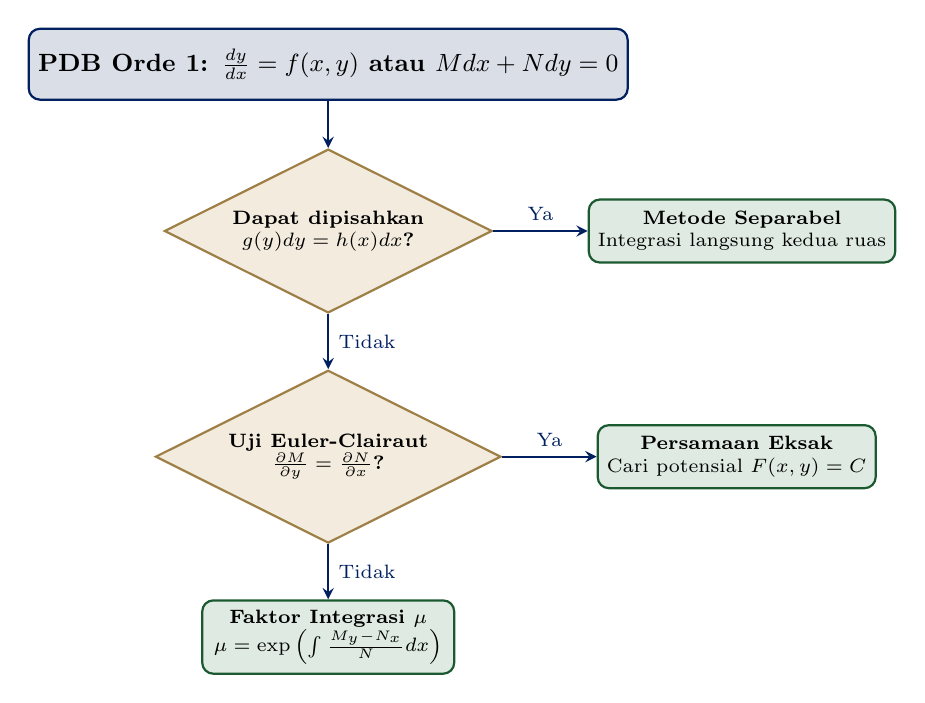
\begin{tikzpicture}[
      node distance=1.1cm and 0.8cm,
      start/.style={rectangle, draw=unibblue, fill=unibblue!15, thick, rounded corners, align=center, font=\small\bfseries, minimum width=4cm, minimum height=0.9cm},
      dec/.style={diamond, draw=unibgold!80!black, fill=unibgold!20, thick, align=center, font=\scriptsize\bfseries, aspect=2},
      action/.style={rectangle, draw=unibgreen!80!black, fill=unibgreen!15, thick, rounded corners, align=center, font=\scriptsize, minimum width=3.2cm, minimum height=0.8cm},
      arrow/.style={->, >=stealth, thick, unibblue}
    ]
      \node[start] (root) {PDB Orde 1: $\frac{dy}{dx} = f(x,y)$ atau $M dx + N dy = 0$};
      \node[dec, below=0.6cm of root] (d1) {Dapat dipisahkan\\$g(y)dy = h(x)dx$?};
      \node[action, right=1.2cm of d1] (a1) {\textbf{Metode Separabel}\\Integrasi langsung kedua ruas};
      
      \node[dec, below=0.7cm of d1] (d2) {Uji Euler-Clairaut\\$\frac{\partial M}{\partial y} = \frac{\partial N}{\partial x}$?};
      \node[action, right=1.2cm of d2] (a2) {\textbf{Persamaan Eksak}\\Cari potensial $F(x,y) = C$};
      
      \node[action, below=0.7cm of d2] (a3) {\textbf{Faktor Integrasi $\mu$}\\$\mu = \exp\left(\int \frac{M_y - N_x}{N} dx\right)$};

      \draw[arrow] (root) -- (d1);
      \draw[arrow] (d1) -- node[above, font=\scriptsize] {Ya} (a1);
      \draw[arrow] (d1) -- node[right, font=\scriptsize] {Tidak} (d2);
      \draw[arrow] (d2) -- node[above, font=\scriptsize] {Ya} (a2);
      \draw[arrow] (d2) -- node[right, font=\scriptsize] {Tidak} (a3);
    \end{tikzpicture}%
    }
  \end{center}
\end{frame}

% FRAME 4: Metode 1 - Separabel
\begin{frame}{Metode 1: Persamaan Separabel (Pemisahan Variabel)}
  \begin{block}{Definisi PDB Terpisahkan}
    Persamaan diferensial orde satu dikatakan \textbf{separabel} jika ruas kanan dapat difaktorkan menjadi perkalian murni fungsi $x$ dan fungsi $y$:
    \begin{equation*}
      \frac{dy}{dx} = g(x) \cdot h(y) \iff \frac{1}{h(y)} dy = g(x) dx
    \end{equation*}
  \end{block}
  \vspace{0.15cm}
  \textbf{Prosedur Penyelesaian Eksplisit:}
  \begin{enumerate}
    \item Kumpulkan semua suku yang memuat variabel terikat $y$ dan diferensial $dy$ di ruas kiri.
    \item Kumpulkan semua suku variabel bebas $x$ dan diferensial $dx$ di ruas kanan.
    \item Lakukan integrasi secara langsung pada kedua sisi:
    \begin{equation*}
      \int \frac{1}{h(y)} dy = \int g(x) dx + C
    \end{equation*}
    \item Selesaikan aljabar untuk menyatakan $y(x)$ secara eksplisit jika memungkinkan.
  \end{enumerate}
\end{frame}

% FRAME 5: Metode 2 - Persamaan Eksak
\begin{frame}{Metode 2: Persamaan Diferensial Eksak}
  \begin{block}{Bentuk Diferensial Total}
    Tinjau persamaan berbentuk diferensial:
    \begin{equation*}
      M(x,y) dx + N(x,y) dy = 0
    \end{equation*}
    Bentuk ini disebut \textbf{Eksak} jika ruas kiri merupakan diferensial total ($dF$) dari suatu fungsi potensial skalar $F(x,y)$:
    \begin{equation*}
      dF = \frac{\partial F}{\partial x} dx + \frac{\partial F}{\partial y} dy = 0 \implies F(x,y) = C
    \end{equation*}
  \end{block}
  \vspace{0.1cm}
  \begin{alertblock}{Teorema Keeksakan Euler-Clairaut}
    Jika $M(x,y)$ dan $N(x,y)$ kontinu dan memiliki turunan parsial pertama kontinu pada domain tertutup, maka syarat perlu dan cukup agar persamaan tersebut eksak adalah:
    \begin{equation*}
      \mathbf{\frac{\partial M}{\partial y} = \frac{\partial N}{\partial x}}
    \end{equation*}
  \end{alertblock}
\end{frame}

% FRAME 6: Medan Konservatif & Fungsi Potensial
\begin{frame}{Intuisi Fisika: Medan Konservatif \& Garis Ekuipotensial}
  \begin{columns}[c]
    \column{0.52\textwidth}
    \textbf{Korelasi dengan Teori Medan Elektromagnetika:}
    \begin{itemize}
      \item Bentuk $M dx + N dy = 0$ merepresentasikan perkalian titik medan vektor gaya elektrostatik $\mathbf{E} = M \hat{i} + N \hat{j}$ dengan elemen lintasan $d\mathbf{r} = dx \hat{i} + dy \hat{j}$:
      \begin{equation*}
        \mathbf{E} \cdot d\mathbf{r} = 0 \iff M dx + N dy = 0
      \end{equation*}
      \item Syarat $\frac{\partial M}{\partial y} = \frac{\partial N}{\partial x}$ ekuivalen dengan kondisi \textbf{Curl Nol} ($\nabla \times \mathbf{E} = 0$).
      \item Solusi umum $F(x,y) = C$ adalah \textbf{Garis Ekuipotensial} elektrostatik bebas pusaran.
    \end{itemize}

    \column{0.44\textwidth}
    \begin{center}
      \resizebox{\linewidth}{!}{%
      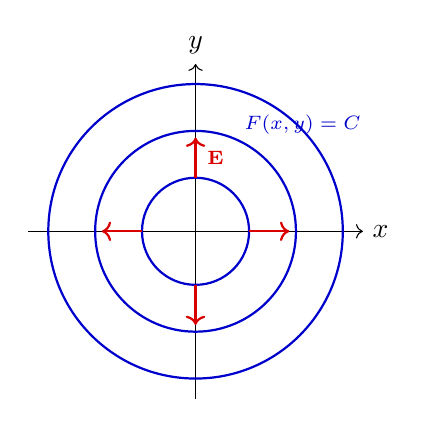
\begin{tikzpicture}[scale=0.85]
        \draw[->] (-2.5,0) -- (2.5,0) node[right] {$x$};
        \draw[->] (0,-2.5) -- (0,2.5) node[above] {$y$};
        % Garis Ekuipotensial
        \draw[blue!80!black, thick] circle (0.8);
        \draw[blue!80!black, thick] circle (1.5);
        \draw[blue!80!black, thick] circle (2.2);
        \node[blue!80!black, font=\scriptsize] at (1.6,1.6) {$F(x,y)=C$};
        % Vektor Medan E
        \draw[->, red!85!black, thick] (0.8,0) -- (1.4,0);
        \draw[->, red!85!black, thick] (0,0.8) -- (0,1.4);
        \draw[->, red!85!black, thick] (-0.8,0) -- (-1.4,0);
        \draw[->, red!85!black, thick] (0,-0.8) -- (0,-1.4);
        \node[red!85!black, font=\scriptsize] at (0.3,1.1) {$\mathbf{E}$};
      \end{tikzpicture}%
      }
    \end{center}
  \end{columns}
\end{frame}

% FRAME 7: Metode 3 - Faktor Pengintegrasi
\begin{frame}{Metode 3: Faktor Pengintegrasi (\textit{Integrating Factor})}
  Jika $M dx + N dy = 0$ \textbf{tidak eksak} ($\frac{\partial M}{\partial y} \neq \frac{\partial N}{\partial x}$), kita dapat mengalikannya dengan fungsi pengali $\mu(x,y)$ sehingga menjadi eksak:
  \begin{equation*}
    \mu M dx + \mu N dy = 0 \implies \frac{\partial (\mu M)}{\partial y} = \frac{\partial (\mu N)}{\partial x}
  \end{equation*}
  \begin{columns}[t]
    \column{0.5\textwidth}
    \begin{block}{Kasus 1: $\mu$ Hanya Fungsi dari $x$}
      Jika $\frac{\frac{\partial M}{\partial y} - \frac{\partial N}{\partial x}}{N} = f(x)$ murni fungsi $x$, maka:
      \begin{equation*}
        \mathbf{\mu(x) = \exp\left( \int f(x) dx \right)}
      \end{equation*}
    \end{block}

    \column{0.5\textwidth}
    \begin{exampleblock}{Kasus 2: $\mu$ Hanya Fungsi dari $y$}
      Jika $\frac{\frac{\partial N}{\partial x} - \frac{\partial M}{\partial y}}{M} = g(y)$ murni fungsi $y$, maka:
      \begin{equation*}
        \mathbf{\mu(y) = \exp\left( \int g(y) dy \right)}
      \end{equation*}
    \end{exampleblock}
  \end{columns}
  \vspace{0.2cm}
  \footnotesize Setelah dikalikan dengan $\mu$, persamaan diselesaikan dengan metode integral potensial eksak standar.
\end{frame}

% FRAME 8: Pemodelan Sirkuit RC dengan CircuiTikZ
\begin{frame}{Pemodelan Fisis: Sirkuit Pengisian Kapasitor RC}
  \begin{columns}
    \column{0.45\textwidth}
    \begin{center}
      \resizebox{\linewidth}{!}{%
      \begin{circuitikz}[american, scale=1.1]
        \draw (0,0) to[battery2, l=$V_0$, invert] (0,2.5)
              to[switch, l=$t{=}0$] (1.8,2.5)
              to[R, l=$R$, v=$v_R$] (3.8,2.5)
              to[C, l=$C$, v=$v_C$] (3.8,0)
              -- (0,0);
        \draw[->, >=stealth, thick, unibblue] (1.8,1.2) arc (160:-160:0.6);
        \node at (2.4,1.2) [unibblue, font=\small\bfseries] {$i(t)$};
      \end{circuitikz}%
      }
    \end{center}
    \vspace{-0.2cm}
    \begin{center}
      \footnotesize Rangkaian RC Seri: Kapasitor Mengisi Energi Medan Listrik.
    \end{center}

    \column{0.55\textwidth}
    \textbf{Formulasi Hukum Kirchhoff:}
    \begin{equation}
      \sum V_{\text{loop}} = 0 \implies v_R(t) + v_C(t) = V_0
    \end{equation}
    Arus pengisian kapasitor diatur oleh laju muatan:
    \begin{equation*}
      i(t) = \frac{dq}{dt} = C \frac{dv_C(t)}{dt}
    \end{equation*}
    Tegangan resistor: $v_R(t) = R \cdot i(t) = R C \frac{dv_C}{dt}$.
    \begin{block}{PDB Standar Pengisian Kapasitor (Orde 1)}
      \begin{equation}
        R C \frac{dv_C}{dt} + v_C(t) = V_0 \iff \frac{dv_C}{dt} + \frac{1}{\tau} v_C = \frac{V_0}{\tau}
      \end{equation}
      dengan konstanta waktu kapasitif $\mathbf{\tau = RC}$ [detik].
    \end{block}
  \end{columns}
\end{frame}

% FRAME 9: Derivasi Solusi Khusus RC
\begin{frame}{Derivasi Analitik Solusi Khusus Tegangan \& Arus RC}
  \textbf{Pemisahan Variabel untuk Pengisian Kapasitor:}
  \begin{equation*}
    R C \frac{dv_C}{dt} = V_0 - v_C \implies \frac{dv_C}{V_0 - v_C} = \frac{1}{R C} dt \implies -\ln|V_0 - v_C| = \frac{t}{RC} + C_1
  \end{equation*}
  Eksponensialkan kedua ruas:
  \begin{equation*}
    V_0 - v_C(t) = A e^{-\frac{t}{RC}} \implies v_C(t) = V_0 - A e^{-\frac{t}{RC}}
  \end{equation*}
  \begin{columns}[t]
    \column{0.5\textwidth}
    \begin{block}{Tegangan Kapasitor ($v_C(0) = 0$)}
      \begin{equation*}
        \mathbf{v_C(t) = V_0 \left(1 - e^{-\frac{t}{\tau}}\right)}
      \end{equation*}
      Tegangan naik secara eksponensial asimtotik mendekati $V_0$.
    \end{block}

    \column{0.5\textwidth}
    \begin{exampleblock}{Arus Pengisian Kapasitor}
      \begin{equation*}
        \mathbf{i(t) = C \frac{dv_C}{dt} = \frac{V_0}{R} e^{-\frac{t}{\tau}}}
      \end{equation*}
      Arus melompat ke $I_0 = \frac{V_0}{R}$ pada $t=0^+$ lalu meluruh menuju nol.
    \end{exampleblock}
  \end{columns}
\end{frame}

% FRAME 10: Dinamika Transien & Paradoks Efisiensi 50%
\begin{frame}{Dinamika Transien \& Paradoks Efisiensi Disipasi 50\%}
  \begin{columns}[c]
    \column{0.52\textwidth}
    \textbf{Neraca Energi Pengisian Kapasitor ($t=0 \to \infty$):}
    \begin{enumerate}
      \item \textbf{Energi Sumber DC:}
      \begin{equation*}
        E_{\text{sumber}} = \int_0^\infty V_0 i(t) dt = \mathbf{C V_0^2}
      \end{equation*}
      \item \textbf{Energi Medan Kapasitor:}
      \begin{equation*}
        E_C = \frac{1}{2} C [v_C(\infty)]^2 = \mathbf{\frac{1}{2} C V_0^2}
      \end{equation*}
      \item \textbf{Energi Disipasi Kalor Resistor:}
      \begin{equation*}
        E_R = \int_0^\infty i(t)^2 R \, dt = \mathbf{\frac{1}{2} C V_0^2}
      \end{equation*}
    \end{enumerate}

    \column{0.46\textwidth}
    \begin{alertblock}{Paradoks Efisiensi 50\%}
      \begin{equation*}
        \eta = \frac{E_C}{E_{\text{sumber}}} = \frac{\frac{1}{2} C V_0^2}{C V_0^2} = \mathbf{50\%}
      \end{equation*}
      Tepat \textbf{separuh} energi sumber terdisipasi menjadi kalor pada resistor! \\
      \vspace{0.1cm}
      Nilai efisiensi ini \textbf{independen dari nilai $R$} (berlaku bahkan jika $R \to 0$, energi hilang via radiasi gelombang EM).
    \end{alertblock}
  \end{columns}
\end{frame}

% FRAME 11: Studi Kasus Snubber RC IGBT
\begin{frame}{Studi Kasus Rekayasa: Proteksi Sakelar IGBT (\textit{RC Snubber})}
  \begin{columns}
    \column{0.45\textwidth}
    \begin{center}
      \resizebox{\linewidth}{!}{%
      \begin{circuitikz}[scale=1.05]
        \draw (0,0) to[battery2, l=$V_{\text{bus}}$, invert] (0,3)
              to[L, l=$L_{\text{beban}}$] (2.8,3) -- (4.2,3);
        % IGBT switch
        \draw (4.2,3) to[normal open switch, l={IGBT}] (4.2,0) -- (0,0);
        % Snubber
        \draw (4.2,3) -- (6.0,3)
              to[R, l=$R_s$] (6.0,1.5)
              to[C, l=$C_s$] (6.0,0) -- (4.2,0);
      \end{circuitikz}%
      }
    \end{center}
    \vspace{-0.2cm}
    \begin{center}
      \footnotesize Rangkaian Snubber RC Paralel Sakelar Daya IGBT.
    \end{center}

    \column{0.55\textwidth}
    \begin{block}{Fenomena Lonjakan Transien Pemutusan}
      Saat sakelar semikonduktor (IGBT/MOSFET) memutus arus induktif, timbul laju lonjakan tegangan transien ekstrem:
      \begin{equation*}
        \frac{dv}{dt} \to \infty
      \end{equation*}
      yang dapat menghancurkan isolasi internal semikonduktor.
    \end{block}
    \begin{exampleblock}{Mitigasi Standar IEEE / IEC}
      Kapasitor snubber $C_s$ menahan laju kenaikan tegangan menjadi nilai aman:
      \begin{equation*}
        \left.\frac{dv}{dt}\right|_{t=0^+} = \frac{I_{\text{peak}}}{C_s} \le \left(\frac{dv}{dt}\right)_{\text{rated}}
      \end{equation*}
    \end{exampleblock}
  \end{columns}
\end{frame}

% FRAME 12: Worked Example Hitungan
\begin{frame}{Contoh Soal Terhitung (Worked Example): Bank Kapasitor}
  \textbf{Kasus Gardu Induk:} Kapasitor bank $C = 200\ \mu\text{F}$ dihubungkan ke bus $V_0 = 250\text{ V}$ melalui resistor pembatas $R = 50\ \Omega$. Kapasitor memiliki tegangan sisa awal $v_C(0) = 50\text{ V}$.
  \vspace{0.15cm}

  \begin{columns}[t]
    \column{0.5\textwidth}
    \textbf{1. Konstanta Waktu Transien $\tau$:}
    \begin{equation*}
      \tau = RC = 50\ \Omega \times (200 \times 10^{-6}\text{ F}) = \mathbf{10\text{ ms}}
    \end{equation*}
    \textbf{2. Persamaan Khusus Tegangan $v_C(t)$:}
    \begin{align*}
      v_C(t) &= V_0 + (v_C(0) - V_0) e^{-t/\tau} \\
      v_C(t) &= 250 - 200 e^{-100t}\quad \text{[Volt]}
    \end{align*}
    \textbf{3. Arus Pemula Transien ($t = 0^+$):}
    \begin{equation*}
      i(0^+) = \frac{V_0 - v_C(0)}{R} = \frac{250 - 50}{50} = \mathbf{4\text{ A}}
    \end{equation*}

    \column{0.5\textwidth}
    \textbf{4. Evaluasi pada $t = 10\text{ ms}$ ($1\tau$) dan $50\text{ ms}$ ($5\tau$):}
    \begin{itemize}
      \item $v_C(10\text{ ms}) = 250 - 200 e^{-1} = \mathbf{176{,}4\text{ V}}$
      \item $v_C(50\text{ ms}) = 250 - 200 e^{-5} = \mathbf{248{,}7\text{ V}}$ ($>99\%$)
      \item $i(10\text{ ms}) = 4 e^{-1} = \mathbf{1{,}47\text{ A}}$
    \end{itemize}
    \textbf{5. Tambahan Energi Medan Listrik:}
    \begin{align*}
      \Delta E_C &= \frac{1}{2} C (V_0^2 - v_C(0)^2) \\
                 &= \frac{1}{2}(200\mu\text{F})(250^2 - 50^2) = \mathbf{6{,}0\text{ Joule}}
    \end{align*}
  \end{columns}
\end{frame}

% FRAME 13: Praktikum Komputasi Julia
% FRAME 13: Praktikum Komputasi Julia
\begin{frame}[fragile]{Praktikum Komputasi Julia: Transien Sirkuit RC}
  \begin{columns}[t]
    \column{0.50\textwidth}
    \begin{block}{Skrip Julia (\texttt{DifferentialEquations.jl})}
\begin{lstlisting}[style=juliastyle]
using DifferentialEquations, Plots

const V0, R, C = 250.0, 50.0, 200e-6
tau = R * C; v0 = 50.0

f_rc(v, p, t) = (V0 - v) / (R * C)
prob = ODEProblem(f_rc, v0, (0.0, 0.06))
sol = solve(prob, Tsit5())

t_vec = 0.0:0.001:0.06
v_an = @. V0 - (V0 - v0) * exp(-t_vec / tau)
plot(sol, label="Tsit5", lw=2, color=:blue)
plot!(t_vec, v_an, label="Eksak", ls=:dash, color=:red)
\end{lstlisting}
    \end{block}

    \column{0.48\textwidth}
    \begin{alertblock}{Visualisasi Respon Transien}
      \centering
      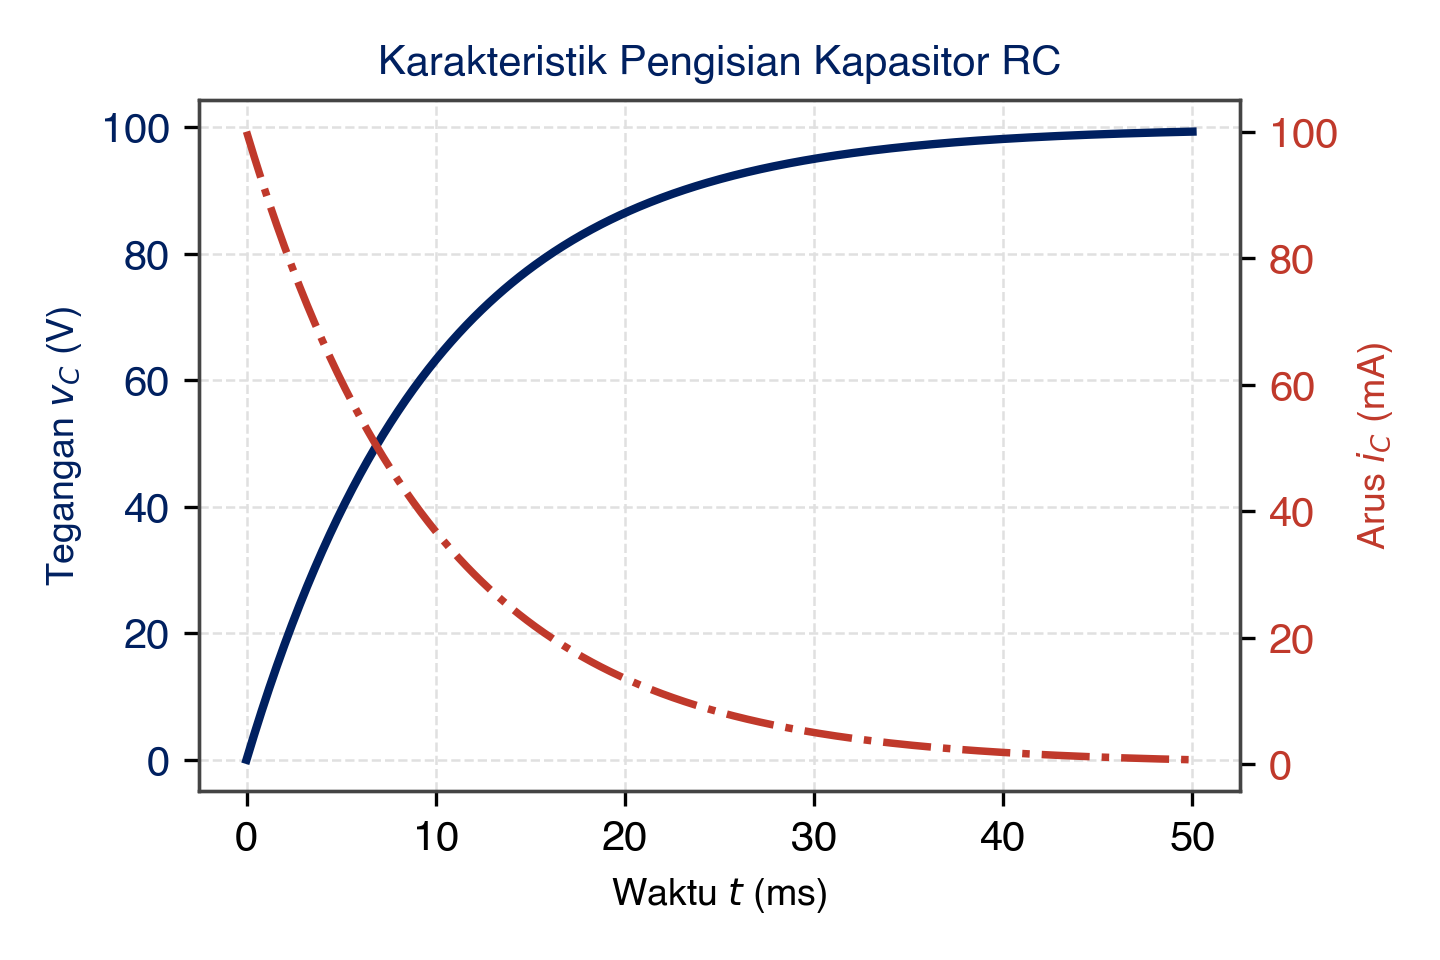
\includegraphics[width=\linewidth, height=0.38\textheight, keepaspectratio]{figures/slides/plot_ch2.png}
    \end{alertblock}
    \vspace{-0.1cm}
    \begin{exampleblock}{Intisari Dinamika Transien}
      \tiny
      Tegangan naik asimtotik ke $250\text{ V}$. Pada $t = \tau = 10\text{ ms}$, tegangan mencapai $63{,}2\%$ rentang transien ($176{,}4\text{ V}$). Arus melonjak $4\text{ A}$ lalu meluruh ke nol.
    \end{exampleblock}
  \end{columns}
\end{frame}

% FRAME 14: Kuis & Tantangan Bloom C1-C6
% FRAME 14: Kuis & Tantangan Bloom C1-C6
\begin{frame}{Kuis Konseptual Interaktif \& Evaluasi Bloom (C1--C6)}
  \begin{columns}[t]
    \column{0.52\textwidth}
    \begin{alertblock}{Peer Instruction: Uji Miskonsepsi Fisik}
      \footnotesize
      \textbf{Kasus Rekayasa:} Kapasitor $C$ diisi dari $0\text{ V}$ hingga $V_0$ via resistor $R$. Jika nilai $R$ diperkecil menjadi setengahnya ($R/2$), energi yang terdisipasi pada resistor ($E_R$) akan:
      \vspace{0.05cm}
      \begin{itemize}\setlength{\itemsep}{1pt}
        \item \textbf{[A]} Menjadi setengahnya karena arus lebih cepat berhenti.
        \item \textbf{[B]} Menjadi dua kali lipat karena arus awal lebih besar.
        \item \textbf{[C]} \textbf{Tetap sama} ($\frac{1}{2} C V_0^2$), tidak bergantung nilai $R$!
        \item \textbf{[D]} Menjadi nol karena resistansi mendekati konduktor ideal.
      \end{itemize}
    \end{alertblock}

    \column{0.46\textwidth}
    \begin{block}{Tantangan Analisis \& Desain (C4--C6)}
      \footnotesize
      \begin{itemize}\setlength{\itemsep}{2pt}
        \item \textbf{C4 (Analisis):} Buktikan daya disipasi puncak resistor terjadi pada $t=0^+$ sebesar $P_{\text{max}} = V_0^2/R$.
        \item \textbf{C5 (Evaluasi):} Evaluasi mengapa efisiensi pengisian kapasitor selalu tepat $50\%$ pada sumber konstan.
        \item \textbf{C6 (Desain):} Rancang snubber $R_s - C_s$ membatasi $dv/dt \le 500\text{ V}/\mu\text{s}$ pada IGBT $25\text{ A}$!
      \end{itemize}
    \end{block}
  \end{columns}
\end{frame}

% FRAME 15: Rangkuman & Penutup
\begin{frame}{Rangkuman Inti Perkuliahan \& Referensi}
  \begin{exampleblock}{Intisari Perkuliahan Minggu 2}
    \begin{itemize}
      \item PDB orde 1 dapat diselesaikan secara sistematis melalui metode separabel, uji keeksakan Euler-Clairaut, atau pengali faktor pengintegrasi $\mu(x)/\mu(y)$.
      \item Solusi persamaan eksak $F(x,y)=C$ merepresentasikan garis ekuipotensial dari medan vektor konservatif ($\nabla \times \mathbf{E} = 0$).
      \item Transien sirkuit RC dicirikan oleh konstanta waktu $\tau = RC$, dengan paradoks efisiensi pengisian tepat $50\%$ terdisipasi menjadi kalor Joule.
    \end{itemize}
  \end{exampleblock}
  \vspace{0.2cm}
  \begin{center}
    \small \textbf{Buku Acuan Utama:} \\
    E. Kreyszig, \textit{Advanced Engineering Mathematics}, 10th ed. | W. Hayt, \textit{Engineering Electromagnetics}. \\
    \vspace{0.3cm}
    \textbf{Tautan Modul \& Bahan Ajar}: \url{https://pd.ndaratha.my.id} \\[0.12cm]\textbf{Video Kuliah (YouTube)}: {\color{red!85!black}\textbf{\url{https://youtu.be/5GQHKrvaSwg}}} \quad \textbar \quad \href{https://www.youtube.com/playlist?list=PLS5oOZWXZeTw}{\color{unibblue}\textbf{Playlist Lengkap}}
  \end{center}
\end{frame}

\end{document}
